\documentclass[aspectratio=169]{beamer}

\usepackage{amsmath, amssymb, amsxtra, amsthm, amsfonts}
\usetheme{moloch}
\usecolortheme{beaver}
\setbeamertemplate{footline}
{
  \leavevmode%
  \hbox{%
    \begin{beamercolorbox}[wd=.5\paperwidth,ht=2.25ex,dp=1ex,center]{author in head/foot}%
      \usebeamerfont{author in head/foot}\insertsection
    \end{beamercolorbox}%
    \begin{beamercolorbox}[wd=.5\paperwidth,ht=2.25ex,dp=1ex,right]{date in head/foot}%
      \usebeamerfont{date in head/foot}\inserttitle\hspace*{2em}
      \insertframenumber{} / \inserttotalframenumber\hspace*{2ex}
    \end{beamercolorbox}}%
  \vskip0pt%
}
\makeatother

\usepackage[english]{babel}
\usefonttheme{serif}

\usepackage{mathtools}
\usepackage{graphicx}
\usepackage{bm}
\usepackage{color}
\usepackage[dvipsnames,table]{xcolor}
\usepackage{tikz}
\usepackage{stanli}
\usepackage{verbatim}
\usepackage{tikz}
\usetikzlibrary{shapes,calc,through,3d,patterns}
\usetikzlibrary{decorations.pathreplacing}
\usetikzlibrary{arrows.meta,calc,positioning}

\usepackage{pgfplots}
\usepackage{siunitx} % For formatting numbers
\usepackage{hyperref}
\hypersetup{colorlinks=true,linkcolor=darkred}
\usepackage{multicol}
\usepackage[absolute,overlay,]{textpos}
\usepackage{pgfplots}
\pgfplotsset{width=10cm,compat=1.9}
\usepackage{subcaption}
\usepackage{multirow}
\usepackage{bbding}
\usepackage{arydshln}
\usepackage{mathtools}
\usepackage{tcolorbox}
\usepackage{animate}

\textblockorigin{80mm}{45mm}


\newtheorem{thm}{Theorem}
\newtheorem{cor}[thm]{Corollary}
\newtheorem{prop}[thm]{Proposition}
\newtheorem{lem}[thm]{Lemma}
\theoremstyle{remark}
\newtheorem*{rem}{Remark}

%Block def
\definecolor{darkred}{rgb}{0.6,0,0}
\setbeamertemplate{blocks}[rounded][shadow=false]
\setbeamercolor{block title}{bg=darkred!15,fg=black}
\setbeamercolor{block body}{bg=darkred!5,fg=black}

\setbeamercolor{itemize item}{fg=darkred}
\setbeamercolor{itemize subitem}{fg=darkred}
\setbeamercolor{itemize subsubitem}{fg=darkred}
\setbeamercolor{enumerate item}{fg=darkred}
\setbeamercolor{button}{bg=gray!30,fg=darkred}

\setbeamertemplate{itemize item}[square]
\setbeamertemplate{itemize subitem}[circle]
\setbeamertemplate{itemize subsubitem}[triangle]
\setbeamertemplate{enumerate items}[circle]
\setbeamercolor{item projected}{bg=darkred}

\newcommand{\bolddelta}{\boldsymbol\delta}
\newcommand{\boldxi}{\boldsymbol\xi}
\DeclareMathOperator*{\A}{\text{\raisebox{-0.2cm}{\Huge A}}}




\title{Analysis of free vibrations}
\subtitle{Analysis of free and forced vibrations}
\author{ME473 Dynamic finite element analysis of structures}
\institute{Stefano Burzio}
\date{2025}

\begin{document}
\usenavigationsymbolstemplate{}
{\setbeamertemplate{footline}{}

  \frame{\titlepage
    \begin{tikzpicture}[overlay, remember picture]
      \node[anchor=north east, xshift=-.9cm] at (current page.north east)
      {
\includegraphics[width=2cm]{../images/epfl_logo.png}};
      \node[anchor=south east, xshift=-.87cm, yshift=.05cm] at (current page.south east)  {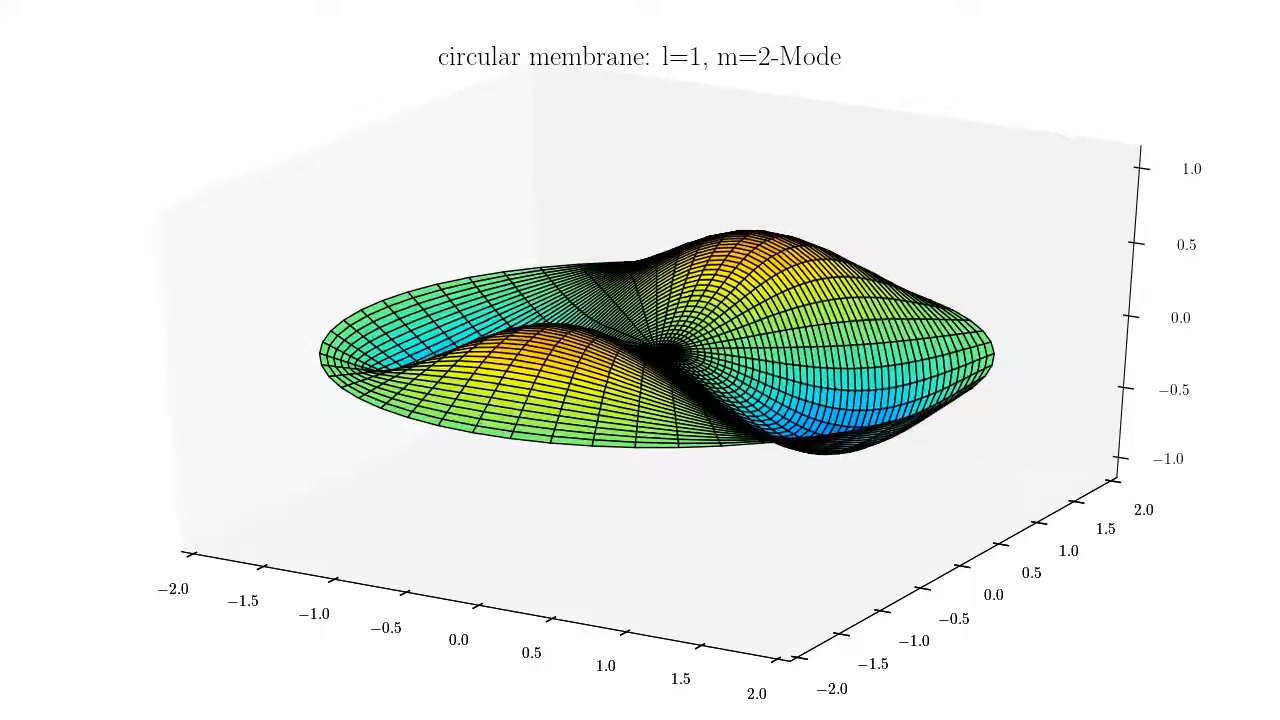
\includegraphics[height=3.7cm]{../images/eigenmodeCircularMembrane.png}};
    \end{tikzpicture}
  }

  \begin{frame}{Where do we stand?}
    \begin{center}
      \begin{tabular}{|c|l|l|l|}
        \hline
        \rowcolor{darkred!20}\textbf{Week} & \textbf{Module}                                & \textbf{Lecture topic}             & \textbf{Mini-projects} \\
        \hline
        1                                  & \multirow{5}{7em}{Linear elastodynamics}       & Strong and weak forms              &                        \\ \cline{1-1} \cline{3-4}
        2                                  &                                                & Galerkin and FE methods            &                        \\ \cline{1-1} \cline{3-4}
        3                                  &                                                & Systematisation of the procedure   & Groups formation       \\ \cline{1-1} \cline{3-4}
        4                                  &                                                & 3d elements, numerical integration & Project 1 statement    \\
        \cline{1-1} \cline{3-4}
        \hline
        5                                  & \multirow{5}{7em}{Special structural elements} & Bars and trusses                   &                        \\
        \cline{1-1} \cline{3-4} 6          &                                                & Beams, frames and grids            &                        \\
        \cline{1-1} \cline{3-4} 7          &                                                & Kirchhoff-Love plates              &                        \\
        \cline{1-1} \cline{3-4}
        8                                  &                                                & Reissner-Mindlin plates            & Project 1 submission   \\
        \cline{1-1} \cline{3-4}
        9                                  &                                                & Shells                             & Project 2 statement    \\
        \hline
        10                                 & \multirow{2}{7em}{Free and forced vibrations}  & Eigenvalue problems                &                        \\
        \cline{1-1} \cline{3-4} 11         &                                                & Analysis of free vibrations        &                        \\
        \hline
      \end{tabular}
    \end{center}
    \vspace{1cm}
  \end{frame}

  \begin{frame}
    \textbf{\large Summary}
    \begin{itemize}
      \item Recap week 10
      \item Numerical modal extraction algorithms for small-scale problems
            \begin{itemize}
              \item Jacobi and generalized Jacobi methods
            \end{itemize}
      \item  Rayleigh-Ritz analysis
      \item Numerical modal extraction algorithms for large-scale problems
            \begin{itemize}
              \item Inverse iteration algorithm
              \item Subspace algorithm
              \item Lanczos algorithm
            \end{itemize}
    \end{itemize}
    \vspace{.5cm}

    \textbf{\large Recommended readings}
    \begin{itemize}
      \item[(H)] Hughes, The finite element method (chap. 10)
      \item[(G)] Gmür, Dynamique des structures (§4.1 and §4.2)
      \item[(P)] Petyt, Introduction to finite element vibration analysis (chap. 11)
      \item[(B)] Bathe, Finite Element Procedures in Engineering Analysis (chap. 11)
    \end{itemize}
  \end{frame}
}

\section{Recap week 10 \\ Eigenvalue problems}
 {\setbeamercolor{background canvas}{bg=darkred!5}
  \setbeamercolor{block body}{bg=darkred!5,fg=black}
  \begin{frame}{Free vibrations of non-rotating conservative systems}
    The discretization of linear three-dimensional elastodynamics, as well as the analysis of vibrations in beams and plates via FEM, all lead to a system of ODE:
    \[
      \mathbf{M} \ddot{\mathbf{q}}(t) + \mathbf{K} \mathbf{q}(t) = \mathbf{r}(t),
    \]
    \begin{columns}[T]
      \begin{column}{.4\textwidth}
        \vspace{-1cm}
        \begin{center}
          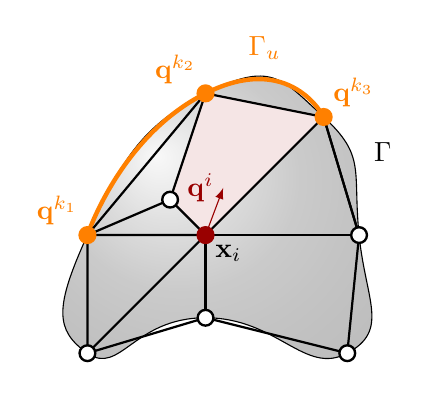
\begin{tikzpicture}[scale=1.5]
            %\draw[step=1.0,black,thin] (0,0) grid (4,4);
            % Draw the potato-like shape
            \shade [ball color= gray!90!black, opacity=.3] plot [thick,smooth cycle, tension=1] coordinates  {(1,2) (2,3.2) (3,3) (3.3,2) (3.2,1) (2,1.3) (1,1)};
            \draw[thin] plot [smooth cycle, tension=1] coordinates {(1,2) (2,3.2) (3,3) (3.3,2) (3.2,1) (2,1.3) (1,1)};
            \draw[ultra thick, orange] plot [smooth, tension=1.3] coordinates {(1,2) (2,3.2) (3,3)};
            \draw[fill=darkred!30,thick,darkred!10] (2,2) -- (3,3) -- (2,3.2) -- (1.7,2.3) -- cycle;
            \node[below right] at (2,2) {$\mathbf x_i$};
            \draw[-latex,darkred] (2,2) -- (2.15,2.4) node[darkred, left]{$\mathbf q^i$};
            % Label the boundary Gamma
            \node at (3.5,2.7) {$\Gamma$};
            \node[orange, above] at (2.5,3.4) {$\Gamma_u$};
            \draw[thick] (1,2) -- (2,3.2) -- (3,3) -- (3.3,2) -- (3.2,1) -- (2,1.3) -- (1,1) -- cycle;
            \draw[thick] (1,2) -- (2,2) -- (3,3) -- (3.3,2);
            \draw[thick] (2,1.3) -- (2,2) -- (3.3,2);
            \draw[thick] (1,1) -- (2,2) -- (1.7,2.3) -- (2,3.2);
            \draw[thick] (1.7,2.3) -- (1,2);
            \node[darkred,draw,shape=circle,fill=darkred,minimum size=2mm,line width=0.3mm,inner sep=0] at (2,2) {};
            \node[draw,shape=circle,fill=white,minimum size=2mm,line width=0.3mm,inner sep=0] at (1,1) {};
            \node[orange,draw,shape=circle,fill=orange,minimum size=2mm,line width=0.3mm,inner sep=0] at (1,2) {};
            \node[draw,shape=circle,fill=white,minimum size=2mm,line width=0.3mm,inner sep=0] at (2,1.3) {};
            \node[orange,draw,shape=circle,fill=orange,minimum size=2mm,line width=0.3mm,inner sep=0] at (2,3.2) {};
            \node[draw,shape=circle,fill=white,minimum size=2mm,line width=0.3mm,inner sep=0] at (1.7,2.3) {};
            \node[orange,draw,shape=circle,fill=orange,minimum size=2mm,line width=0.3mm,inner sep=0] at (3,3) {};
            \node[draw,shape=circle,fill=white,minimum size=2mm,line width=0.3mm,inner sep=0] at (3.2,1) {};
            \node[draw,shape=circle,fill=white,minimum size=2mm,line width=0.3mm,inner sep=0] at (3.3,2) {};
            \node[orange,above left] at (1,2) {$\mathbf q^{k_1}$};
            \node[orange,above left] at (2,3.2) {$\mathbf q^{k_2}$};
            \node[orange,above right] at (3,3) {$\mathbf q^{k_3}$};
          \end{tikzpicture}
        \end{center}
      \end{column}
      \begin{column}{.65\textwidth}
        \vspace{-0.9cm}
        \begin{block}{}
          \textbf{Free vibration:} no external forcing is applied, i.e.   $\mathbf{r}(t) = \mathbf{0}.$
        \end{block}
        \begin{itemize}
          \item Generalized nodal displacements: $$\mathbf q(t)=[\mathbf q^1(t),\dots, \mathbf q^n(t)]^T.$$
          \item \textbf{Boundary conditions:} $\mathbf q^k=\hat{\mathbf q}^k$ for all $k$ such that $\mathbf x_k\in\Gamma_u$.
          \item  \textbf{Initial conditions:} $\mathbf q(0)=\mathbf u_0$ and $\dot{\mathbf q}(0)=\mathbf v_0$
        \end{itemize}
      \end{column}
    \end{columns}
  \end{frame}

  \begin{frame}
    \begin{columns}
      \begin{column}{0.42\textwidth}
        \vspace{-0.3cm}
        \begin{center}
          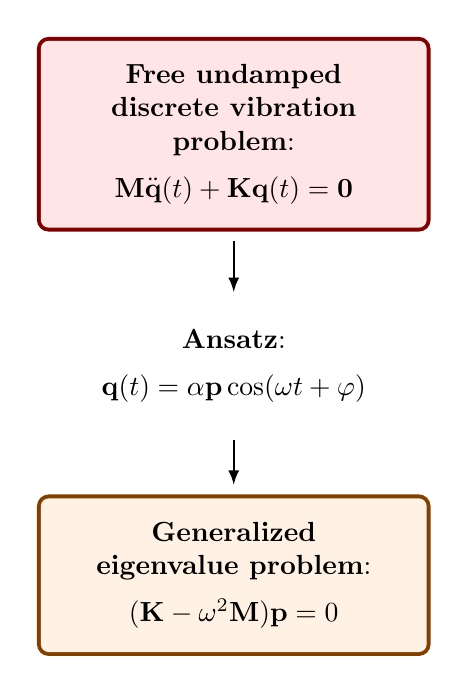
\begin{tikzpicture}[scale=0.7]
            \node (dvp) at (0,6) {
              \begin{tcolorbox}[colframe=red!50!black, colback=red!10, coltitle=black, rounded corners,width=5cm]
                \centering \textbf{Free undamped discrete vibration problem}: \\[5pt] $\mathbf{M} \ddot{\mathbf{q}}(t) + \mathbf{K} \mathbf{q}(t) = \mathbf{0}$
              \end{tcolorbox}
            };
            \node (ans) at (0,1.8) {
              \begin{tcolorbox}[colframe=white, colback=white, coltitle=black, rounded corners, width=5cm]
                \centering \textbf{Ansatz}: \\[5pt] $\mathbf q(t)=\alpha \mathbf p \cos(\omega t+\varphi)$
              \end{tcolorbox}
            };
            \node (gep) at (0,-2) {
              \begin{tcolorbox}[colframe=orange!50!black, colback=orange!10, coltitle=black, rounded corners,width=5cm]
                \centering \textbf{Generalized eigenvalue problem}: \\[5pt] $(\mathbf{K} - \omega^2 \mathbf{M}) \mathbf{p} = 0$
              \end{tcolorbox}
            };
            % Drawing arrows
            \draw[-latex, thick] (dvp.south) -- (ans.north);
            \draw[-latex, thick] (ans.south) -- (gep.north);
          \end{tikzpicture}
        \end{center}
      \end{column}
      \begin{column}{0.54\textwidth}
        \textbf{Solving the eigenvalue problem:}
        $$n=\text{dim}(\mathbf K)=\text{dim}(\mathbf M)$$
        There are $n$ eigenvalues $\lambda_j$ and $n$ corresponding eigenvectors $\mathbf p_j$ such that:
        \begin{block}{}
          \textbf{Eigenvalues} (\emph{natural frequencies} squared): $\lambda_j=\omega_j^2$ are the roots of the characteristic polynomial:
          $$\text{det}(\mathbf K-\lambda\mathbf M)=0.$$
        \end{block}
        \begin{block}{}
          \textbf{Eigenvectors} (\emph{modal shapes}): $\mathbf p_j$ are the solution of the equation
          $$(\mathbf{K} - \lambda_j \mathbf{M})\mathbf p_j=\mathbf 0.$$
        \end{block}
      \end{column}
    \end{columns}
  \end{frame}

  \begin{frame}{Rigid body modes}
    In the semi-discrete weak form obtained via finite element discretization:
    \begin{itemize}
      \item The \textbf{mass matrix} \( \mathbf{M} \) is symmetric and strictly positive definite.
      \item The \textbf{stiffness matrix} \( \mathbf{K} \) is symmetric and positive semi-definite:
            \[
              \mathbf{K} \mathbf{p} = \mathbf{0} \quad \text{for certain nonzero vectors } \mathbf{p}.
            \]
    \end{itemize}
    Consequently, the eigenvalues \( \lambda_j\) of the generalized eigenvalue problem are \textbf{all real and non-negative}:
    \[
      0 \,\leq\, \omega_1 \leq \omega_2 \leq \dots \leq \omega_n.
    \]
    \begin{tcolorbox}[colback=darkred!10,colframe=darkred!40!black]
      \textbf{Rigid body modes:} zero eigenvalues (i.e., \( \omega_j = 0 \)) correspond to \emph{rigid body motions}, where the system undergoes displacement without internal deformation.
    \end{tcolorbox}
  \end{frame}

  \begin{frame}{Orthonormalization of mode shapes}
    \small
    \begin{block}{}
      Let $\mathbf p_i$ and $\mathbf p_j$ two eigenvectors corresponding to the  eigenvalues $\lambda_i$ and $\lambda_j$, then
      $$
        \mathbf p_i^T\mathbf M\mathbf p_j  =\delta_{ij}
        \qquad\text{and}\qquad
        \mathbf p_i^T\mathbf K\mathbf p_j  =\omega_i^2\delta_{ij}
      $$
      where $\delta_{ij}$ represent Kronecker symbol.
    \end{block}
    \begin{tcolorbox}[colback=darkred!10,colframe=darkred!40!black]
      We organize the modal vectors $\mathbf p_i$ in a so-called \textbf{modal matrix} $\mathbf P$:
      $$\mathbf P=\left[ \begin{array}{c;{2pt/2pt}c;{2pt/2pt}c;{2pt/2pt}c}
            \mathbf p_{1} & \mathbf p_{2} & \dots & \mathbf p_{n} \\
          \end{array}\right]$$
      then
      $$  \mathbf P^T\mathbf M\mathbf P  =\mathbf I       \qquad\text{and}\qquad
        \mathbf P^T\mathbf K\mathbf P  =\mathbf\Lambda$$
      where $\mathbf I$ is the identity matrix of order $n$ and $\mathbf\Lambda$ the \textbf{spectral matrix}:
      $$\mathbf\Lambda=\text{diag}(\lambda_1,\dots,\lambda_n)=\text{diag}(\omega_1^2,\dots,\omega_n^2).$$
    \end{tcolorbox}
  \end{frame}


  \begin{frame}{Small and large scale generalized eigenvalue problems}
    \small We are interested in economical computational algorithms for extracting eigenpairs $(\lambda_j,\mathbf p_j)$ of the generalized eigenvalue problem :
    $$(\mathbf K - \lambda \mathbf{M})\mathbf p=\mathbf 0$$
    \vspace{-0.8cm}
    \begin{columns}[T,onlytextwidth]
      \begin{column}{.48\textwidth}
        \begin{block}{}
          \textbf{\centering Small-scale problems}
          \begin{itemize}
            \item Matrices are of modest size $n\leq 250$ or $250\leq n \leq 2500$ and small bandwidth matrices.
            \item An explicit reduction to standard eigenvalue form is typically employed.
            \item The most effective algorithms are:
                  \begin{enumerate}
                    \item Rayleigh quotient minimization,
                    \item Generalized Jacobi method,
                    \item Householder-QR method.
                  \end{enumerate}
          \end{itemize}
        \end{block}
      \end{column}
      \begin{column}{.48\textwidth}
        \begin{block}{}
          \textbf{Large-scale problems}
          \begin{itemize}
            \item $n\geq 2500$.
            \item The most effective algorithms are :
                  \begin{enumerate}
                    \item Subspace iteration,
                    \item Lanczos' method,
                    \item Guyan-Irons method,
                    \item Arnoldi Davidson methods.
                  \end{enumerate}
          \end{itemize}
        \end{block}
      \end{column}
    \end{columns}
  \end{frame}

  \begin{frame}{Small-scale modal extraction via the Rayleigh quotient}
    \small
    For a trial shape $\mathbf w\ne\mathbf 0$, the Rayleigh quotient estimates the squared angular frequency:
    \[
      \mathcal R(\mathbf w)=
      \frac{\mathbf w^T\mathbf K\mathbf w}{\mathbf w^T\mathbf M\mathbf w},
      \qquad \lambda_1\leq\mathcal R(\mathbf w)\leq\lambda_n .
    \]
    At each mode shape $\mathbf p_j$, the quotient is stationary and
    $\mathcal R(\mathbf p_j)=\lambda_j=\omega_j^2$.
    \begin{block}{Extracting modes in ascending order}
      \begin{enumerate}
        \item Minimize $\mathcal R(\mathbf w)$ over all nonzero trial shapes to obtain $\lambda_1$.
        \item For mode $j>1$, minimize over shapes mass-orthogonal to all earlier modes:
              \[
                \lambda_j=\min_{\substack{\mathbf w\ne\mathbf 0\\
                    \mathbf w^T\mathbf M\mathbf p_i=0,\ i=1,\ldots,j-1}}\mathcal R(\mathbf w).
              \]
      \end{enumerate}
      At each step, mass-normalize the minimizing shape to obtain $\mathbf p_j$.
      It satisfies $\mathbf K\mathbf p_j=\lambda_j\mathbf M\mathbf p_j$.
    \end{block}
  \end{frame}
 }

\section[Numerical modal extraction algorithms for small-scale problems]{Numerical modal extraction algorithms}

\begin{frame}{Generalized Jacobi method}
  \small
  Consider a \emph{small}, dense pair of matrices $(\mathbf K,\mathbf M)$ of order $q$, with $\mathbf K$ and $\mathbf M$ both symmetric and positive definite matrices.
  We seek all $q$ modal pairs $(\lambda_j,\mathbf p_j)$ for $j=1,\dots q$.
  \begin{block}{\small Why use Jacobi instead of repeated Rayleigh minimization?}
    \begin{itemize}
      \item Rayleigh minimization first gives $\lambda_1$ and $\mathbf p_1$, then to obtain mode $j$ requires solving repeated constrained minimization problems
            $$\min_{\mathbf w^T\mathbf M\mathbf p_i=0,\ i<j}\mathcal R(\mathbf w).$$
            Each additional mode introduces another mass-orthogonality constraint.
      \item Generalized Jacobi applies a two-coordinate change of basis to both matrices at each pivot. It zeros the chosen stiffness and mass couplings together. When convergence is reached, all modes are obtained together:
            \[
              \mathbf P^T\mathbf K\mathbf P=\mathbf\Lambda,
              \qquad \mathbf P^T\mathbf M\mathbf P=\mathbf I,
            \]
    \end{itemize}
  \end{block}
\end{frame}

\begin{frame}{Transformation methods}
  \small
  Start with $\mathbf K_0=\mathbf K$, $\mathbf M_0=\mathbf M$ and
  $\mathbf P_0=\mathbf I$. Produce a sequence of matrices $\mathbf K_k$, $\mathbf M_k$ such that
  $$\mathbf K_k\to \mathbf \Lambda,\quad  \mathbf M_k\to \mathbf I  \quad\mbox{and}\quad \mathbf P_k\to \mathbf P\quad\mbox{as } k \to \infty$$
  \vspace{-0.4cm}
  \begin{enumerate}
    \item Choose a change of basis $\mathbf J_k$ to eliminate a coupling.
          Apply it to both matrices and update the basis:
          \[
            \mathbf K_k=\mathbf J_k^T\mathbf K_{k-1}\mathbf J_k,\quad
            \mathbf M_k=\mathbf J_k^T\mathbf M_{k-1}\mathbf J_k,\quad
            \mathbf P_k=\mathbf P_{k-1}\mathbf J_k .
          \]
          The transformations $\mathbf J_k$ are selected to bring $\mathbf K_k$ and $\mathbf M_k$ closer to diagonal form.
    \item Stop when both matrices are diagonal up to a tolerance. With $\mathbf P_\ell=\mathbf J_1\cdots\mathbf J_\ell$,
          \[
            \mathbf P_\ell^T\mathbf K\mathbf P_\ell\approx\mathbf D_K,\qquad
            \mathbf P_\ell^T\mathbf M\mathbf P_\ell\approx\mathbf D_M ,
          \]
  \end{enumerate}
  \vspace{-0.2cm}
  \begin{block}{Recover the modal pairs}
    For column $\mathbf p_j$ of $\mathbf P_\ell$, mass normalization gives approximated mode shapes and approximated eigenvalues:
    \vspace{-0.2cm}
    $$\mathbf p_j/\sqrt{(\mathbf D_M)_{jj}}\quad\mbox{and}\quad \lambda_j\approx(\mathbf D_K)_{jj}/(\mathbf D_M)_{jj}.$$
  \end{block}
\end{frame}

\begin{frame}{Jacobi method for a symmetric eigenproblem}
  \small
  When $\mathbf M=\mathbf I$, the modal problem becomes
  $\mathbf K\mathbf p_j=\lambda_j\mathbf p_j$. We seek an orthonormal modal basis for which
  \[
    \mathbf P^T\mathbf K\mathbf P=\mathbf\Lambda,
    \qquad \mathbf P^T\mathbf P=\mathbf I .
  \]
  \vspace{-0.3cm}
  \begin{block}{\small Build the modal basis two entries at a time}
    Start with $\mathbf K_0=\mathbf K$ and $\mathbf P_0=\mathbf I$.
    For a pair $i<j$, choose an orthogonal rotation $\mathbf J_1$ so that for the updated matrix
    $$\mathbf K_1=\mathbf J_1^T\mathbf K_0\mathbf J_1$$
    we have zeros in the off diagonal elements ${k_1}_{ij}=0$. Update the change of basis:
    \[
      \mathbf K_1=\mathbf J_1^T\mathbf K_{0}\mathbf J_1,
      \qquad \mathbf P_1=\mathbf P_{0}\mathbf J_1 .
    \]
  \end{block}
  After $k$ iterations, $\mathbf K_k$ approaches a diagonal form, its diagonal gives the eigenvalues
  $$\mathbf K_k=\mathbf J_k^T\dots \mathbf J_{1}^T \mathbf K\mathbf J_1\dots\mathbf J_k$$
  and $\mathbf P_k=\mathbf J_1\dots\mathbf J_k$ approximate the modal matrix.
\end{frame}

\begin{frame}{Choosing the Jacobi rotation}
  \small
  The $q\times q$ rotation $\mathbf J_{k}(\theta)$ acts in the $(i,j)$ plane
  and leaves every other coordinate unchanged.
  \vspace{0.2cm}
  \begin{columns}[c,onlytextwidth]
    \begin{column}{.53\textwidth}
      \centering
      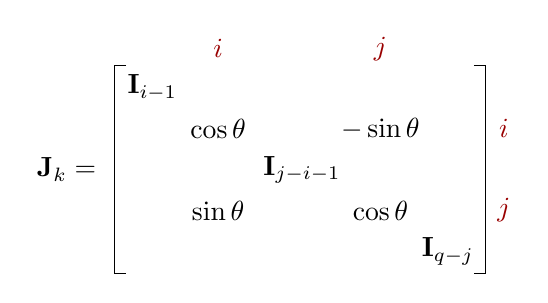
\begin{tikzpicture}[x=0.95cm,y=0.52cm]
        \node[anchor=east] at (-0.02,2) {$\mathbf J_{k}=$};
        \draw (0.25,4.55)--(0.10,4.55)--(0.10,-0.55)--(0.25,-0.55);
        \draw (4.90,4.55)--(5.05,4.55)--(5.05,-0.55)--(4.90,-0.55);
        \node at (0.60,4) {$\mathbf I_{i-1}$};
        \node at (2.60,2) {$\mathbf I_{j-i-1}$};
        \node at (4.55,0) {$\mathbf I_{q-j}$};
        \node at (1.48,3) {$\cos\theta$};
        \node at (3.65,3) {$-\sin\theta$};
        \node at (1.48,1) {$\sin\theta$};
        \node at (3.65,1) {$\cos\theta$};
        \node[darkred] at (1.48,4.95) {$i$};
        \node[darkred] at (3.65,4.95) {$j$};
        \node[darkred] at (5.30,3) {$i$};
        \node[darkred] at (5.30,1) {$j$};
      \end{tikzpicture}
    \end{column}
    \begin{column}{.44\textwidth}
      \small For $k_{ij}\ne0$ and $k_{ii}\ne k_{jj}$,
      \[
        \tan(2\theta)=\frac{2k_{ij}}{k_{ii}-k_{jj}},
        \qquad |\theta|\leq\pi/4 .
      \]
      If $k_{ii}=k_{jj}$, take $\theta=\pi/4$.
    \end{column}
  \end{columns}
  \vspace{0.2cm}
  \begin{block}{Transformed off-diagonal entry}
    \[
      k_{ij}\gets k_{ij}\cos(2\theta)
      -\tfrac12(k_{ii}-k_{jj})\sin(2\theta).
    \]
  \end{block}
\end{frame}

\begin{frame}{From a rotation to a threshold Jacobi sweep}
  \small
  One \textbf{sweep} visits all pairs $i<j$ in row order. Later rotations may
  reintroduce a coupling eliminated earlier.
  \begin{enumerate}
    \item For the positive-definite stiffness matrix, measure
          the coupling relative to the two diagonal entries:
          \[
            c_{ij}=\frac{|k_{ij}|}{\sqrt{k_{ii}k_{jj}}}.
          \]
    \item In sweep $m=1,2,\ldots$, rotate only if $c_{ij}>10^{-2m}$.
          Sweep~1 removes the larger couplings first; subsequent sweeps use a lower threshold.
    \item After a sweep, check that all couplings are small and that the
          diagonal estimates have stabilized. Sort the final diagonal values
          and apply the same permutation to the columns of $\mathbf P$.
  \end{enumerate}
\end{frame}

\begin{frame}{MATLAB example - the Jacobi method}
  \begin{center}
    \href{https://drive.mathworks.com/sharing/6a9792ef-d0a7-4aca-a1d0-8b1862b0ac3b}{\beamergotobutton{Go to Matlab Drive}}
  \end{center}
\end{frame}

\begin{frame}{From standard to generalized Jacobi}
  \small
  A pivot still acts on two coordinates $i,j$. What changes is the
  condition that the new basis vectors must satisfy.
  \begin{columns}[T,onlytextwidth]
    \begin{column}{.48\textwidth}
      \begin{block}{\small Standard problem: $\mathbf M=\mathbf I$}
        An orthogonal rotation preserves mass:
        \[
          \mathbf J_k^T\mathbf I\,\mathbf J_k=\mathbf I .
        \]
        Choose one angle $\theta$ to zero the stiffness entry
        $(\mathbf K_k)_{ij}$.
      \end{block}
    \end{column}
    \begin{column}{.48\textwidth}
      \begin{block}{\small Generalized problem:  $\mathbf M \neq \mathbf I$}
        The same change of basis acts on stiffness and mass. Choose
        $\mathbf J_k$ to satisfy two conditions:
        \[
          (\mathbf K_k)_{ij}=(\mathbf M_k)_{ij}=0 .
        \]
        The new directions are mass-orthogonal.
      \end{block}
    \end{column}
  \end{columns}
  \medskip
  \textbf{Why can one angle be insufficient?}
  Even if the current mass block is diagonal, an ordinary rotation produces
  $m'_{ij}=(m_{jj}-m_{ii})\sin\theta\cos\theta$.
  Unequal diagonal masses can therefore acquire a coupling.
\end{frame}

\begin{frame}{Choosing the generalized Jacobi transformation}
  \small
  Start with $\mathbf K_0=\mathbf K$, $\mathbf M_0=\mathbf M$ and $\mathbf P_0=\mathbf I$. At step $k$, choose a pivot pair $i<j$.
  \vspace{0.2cm}
  \begin{columns}[c,onlytextwidth]
    \begin{column}{.53\textwidth}
      \centering
      \begin{tikzpicture}[x=0.95cm,y=0.52cm]
        \node[anchor=east] at (-0.02,2) {$\mathbf J_{k}=$};
        \draw (0.25,4.55)--(0.10,4.55)--(0.10,-0.55)--(0.25,-0.55);
        \draw (4.90,4.55)--(5.05,4.55)--(5.05,-0.55)--(4.90,-0.55);
        \node at (0.60,4) {$\mathbf I_{i-1}$};
        \node at (2.60,2) {$\mathbf I_{j-i-1}$};
        \node at (4.55,0) {$\mathbf I_{q-j}$};
        \node at (1.48,3) {$1$};
        \node at (3.65,3) {$\alpha$};
        \node at (1.48,1) {$\gamma$};
        \node at (3.65,1) {$1$};
        \node[darkred] at (1.48,4.95) {$i$};
        \node[darkred] at (3.65,4.95) {$j$};
        \node[darkred] at (5.30,3) {$i$};
        \node[darkred] at (5.30,1) {$j$};
      \end{tikzpicture}
    \end{column}
    \begin{column}{.46\textwidth}
      Choose $\alpha$ and $\gamma$ to eliminate both pivot entries in $\mathbf K_k$ and $\mathbf M_k$:
      \[
        \begin{aligned}
          k_{ii}\alpha+k_{jj}\gamma+k_{ij}(1+\alpha\gamma) & =0,  \\
          m_{ii}\alpha+m_{jj}\gamma+m_{ij}(1+\alpha\gamma) & =0 .
        \end{aligned}
      \]
      For $\mathbf M_{k-1}=\mathbf I$, $\alpha=-\gamma$.
      Normalizing the pivot columns recovers the standard rotation
      with $\gamma=\tan\theta$.
    \end{column}
  \end{columns}
  \begin{block}{\small Update at step $k$}
    As for the standard Jacobi method :
    \[
      \mathbf K_k=\mathbf J_k^T\mathbf K_{k-1}\mathbf J_k,\quad
      \mathbf M_k=\mathbf J_k^T\mathbf M_{k-1}\mathbf J_k,\quad
      \mathbf P_k=\mathbf P_{k-1}\mathbf J_k .
    \]
  \end{block}
\end{frame}

\begin{frame}{Generalized Jacobi sweeps and computational cost}
  \small
  A sweep visits $q(q-1)/2$ pairs. For a positive-definite pair, apply
  the pivot if either scaled coupling exceeds the sweep threshold:
  \[
    c^K_{ij}=\frac{|k_{ij}|}{\sqrt{k_{ii}k_{jj}}},\qquad
    c^M_{ij}=\frac{|m_{ij}|}{\sqrt{m_{ii}m_{jj}}}.
  \]
  Later pivots can reintroduce couplings. Stop when both sets are small
  and the stiffness-to-mass ratios have stabilized.
  \begin{block}{\small Recover the modal pairs after the last step $\ell$}
    \[
      \lambda_j\simeq\frac{(\mathbf K_\ell)_{jj}}{(\mathbf M_\ell)_{jj}},\qquad
      \mathbf p_j=\frac{\mathbf P_\ell(:,j)}{\sqrt{(\mathbf M_\ell)_{jj}}}.
    \]
    Sort the eigenvalues in ascending order and reorder the mode shapes.
  \end{block}
  Each pivot updates two rows or columns at a cost of $O(q)$.
  For a dense pair of order $q$, $s$ full sweeps cost $O(sq^3)$ work
  and require $O(q^2)$ storage.
\end{frame}

\begin{frame}{Accuracy of the generalized Jacobi solution}
  \small
  \begin{itemize}
    \item \textbf{Standard Jacobi.} For symmetric $\mathbf K$, cyclic row sweeps with
          $|\theta|\leq\pi/4$ drive $S(\mathbf K)=\sum_{r\ne s}k_{rs}^2$ to zero.
          Each rotation reduces $S$ by $2k_{ij}^2$, even if earlier couplings reappear.
    \item \textbf{Generalized Jacobi.} For symmetric $\mathbf K$ and $\mathbf M$ symmetric and positive-definite, global convergence depends on the transformation and pivot order.
          With simple eigenvalues, cyclic Falk--Langemeyer sweeps converge
          quadratically to a near diagonal form.
  \end{itemize}
  \begin{block}{\small Check the computed modes against the original matrices}
    \[
      \mathbf r_j=\mathbf K\mathbf p_j-\lambda_j\mathbf M\mathbf p_j,\qquad
      \eta_j=\frac{\|\mathbf r_j\|_2}
      {(\|\mathbf K\|_2+|\lambda_j|\,\|\mathbf M\|_2)\,\|\mathbf p_j\|_2}.
    \]
    Check $\eta_j$ for every mode and $\|\mathbf P^T\mathbf M\mathbf P-\mathbf I\|_2$
    against the chosen tolerances.
  \end{block}
\end{frame}

\begin{frame}{MATLAB example - the generalized Jacobi method}
  \begin{center}
    \href{https://drive.mathworks.com/sharing/6a9792ef-d0a7-4aca-a1d0-8b1862b0ac3b}{\beamergotobutton{Go to Matlab Drive}}
  \end{center}
\end{frame}

\section{Rayleigh-Ritz analysis}

\begin{frame}{Rayleigh-Ritz analysis: fundamentals}
  \begin{block}{}
    \textbf{Goal:} approximate the lowest $n_{modes}$ eigenvalues and corresponding eigenvectors of the generalized eigenproblem \( \mathbf K\mathbf p = \lambda\mathbf M \mathbf p \) of \emph{large} order $n$.
  \end{block}

  \textbf{Inputs:}
  \begin{itemize}
    \item \(\mathbf K \), \(\mathbf M \): positive definite stiffness and mass matrices (or shifted to be so). If $\mathbf K$ is singular, use shift: set \( \mathbf K_\sigma =\mathbf K + \sigma\mathbf M \) with \( \sigma > 0 \).
    \item $n_{modes}$ linearly independent \textbf{Ritz basis vectors} $\boldsymbol{\psi}_i$, spanning a subspace $\mathcal S$.
  \end{itemize}

  \textbf{Output:}
  \begin{itemize}
    \item Approximated modal matrix of size $n\times n_{modes}$
          $$\mathbf P=[\mathbf p_1,\dots,\mathbf p_{n_{modes}}]$$
    \item Approximated spectral matrix: $$\mathbf \Lambda=\text{diag}(\lambda_1,\dots,\lambda_{n_{modes}})$$
  \end{itemize}
\end{frame}


\begin{frame}{Rayleigh-Ritz reduction algorithm}
  \small \begin{enumerate}
    \item Any trial vector in $\mathcal S$ is written as
          \(
          \mathbf w = \sum_{i=1}^{n_{modes}} x_i \boldsymbol{\psi}_i ,
          \)
          with coordinates $x_i$.
    \item Insert $\mathbf w = \mathbf \Psi \mathbf x$ into $\mathcal R(\mathbf w)$ to obtain the projected stiffness and mass matrices into the Ritz basis:
          \[
            {\mathbf K}^* = \mathbf \Psi^T \mathbf K \mathbf \Psi, \qquad {\mathbf M}^* = \mathbf \Psi^T \mathbf M \mathbf \Psi,
          \]
          where $\mathbf \Psi = [\boldsymbol{\psi}_1, \boldsymbol{\psi}_2, \dots, \boldsymbol{\psi}_{n_{modes}}]$.
    \item Solve the \emph{small} reduced $(n_{modes}\times n_{modes})$ generalized eigenvalue problem by minimization:
          \[
            {\mathbf K}^* \mathbf p^* = \lambda^*\, {\mathbf M}^* \mathbf p^* .
          \]
          to obtain approximate eigenpairs $(\lambda^*_i, \mathbf p_i^*)$   for \( i = 1, 2, \dots, n_{modes} \). $\lambda^*_i$ are \textbf{Ritz values} and  $\mathbf p^*_i$ are \textbf{Ritz vectors}.
    \item Compute the modal and the spectral matrices:
          \[
            {\mathbf \Lambda} = \text{diag}(\lambda^*_1, \lambda^*_2, \dots, \lambda^*_{n_{modes}}) ,
          \]
          and the approximate mode shapes
          \[
            \mathbf p_i = \mathbf \Psi \mathbf p_i^* .
          \]
  \end{enumerate}
\end{frame}

\begin{frame}{Practical aspects and remarks}
  \begin{tcolorbox}[colback=darkred!10,colframe=darkred!40!black]
    \textbf{Upper-bound property}:
    \[
      \lambda_i \le \lambda_i^* , \qquad i=1,\dots,n_{modes} .
    \]
  \end{tcolorbox}
  \begin{itemize}
    \item Ritz basis often obtained from static solutions:
          \[
            \mathbf K \mathbf \Psi = \mathbf L,
          \]
          where $\mathbf L$ contains chosen load patterns.
    \item Accuracy depends on how well $\mathcal S$ approximates the
          subspace of the lowest eigenmodes.
    \item Many well-known methods are special cases of Rayleigh--Ritz procedure:
          \begin{itemize}
            \item \textbf{Static condensation} (Irons-Guyan reduction)
            \item \textbf{Subspace iteration}
            \item \textbf{Lanczos algorithm}
          \end{itemize}
  \end{itemize}
\end{frame}


\section{Inverse iteration algorithm}

\begin{frame}{General idea of inverse and forward iteration}
  \vspace{-0.2cm}
  \small
  \begin{block}{}
    \textbf{Goal:} compute \textbf{one} eigenvector of the generalized eigenproblem \( \mathbf K\mathbf p = \lambda\mathbf M \mathbf p \).
  \end{block}
  \textbf{Idea:} Use an \emph{iterative} improvement of an assumed eigenvector.
  \begin{itemize}
    \item Start from an arbitrary vector $\mathbf p^{(0)}$.
    \item Generate a sequence of vectors $\mathbf p^{(1)}, \mathbf p^{(2)}, \dots$ that converge to an eigenvector.
    \item  Compute an approximate eigenvalue using Rayleigh's quotient:
          \[
            \lambda^{(k)} = \mathcal R(\mathbf p^{(k)}).
          \]
  \end{itemize}
  \begin{columns}[T]
    \begin{column}{0.5\textwidth}
      \textbf{Inverse iteration:}
      \begin{itemize}
        \item Form a \emph{“force”} vector:
              \(
              \boldsymbol \ell_1 = \mathbf M \mathbf p^{(0)}.
              \)
        \item Solve the static-like equilibrium problem:
              \[
                \mathbf K \mathbf p^{(1)} = \boldsymbol \ell_1,
              \]
        \item Repeat until convergence is met.
      \end{itemize}
    \end{column}
    \begin{column}{0.5\textwidth}
      \textbf{Forward iteration:}
      \begin{itemize}
        \item Compute $\boldsymbol \ell_1 = \mathbf K \mathbf p^{(0)}$.
        \item Solve
              \[
                \mathbf M \mathbf p^{(1)} = \boldsymbol \ell_1 ,
              \]
        \item Repeat until convergence is met.
      \end{itemize}
    \end{column}
  \end{columns}
\end{frame}


\begin{frame}{Inverse iteration algorithm}
  \small
  \textbf{Inputs:}
  \vspace{-0.3cm}
  \begin{multicols}{2}
    \begin{itemize}
      \item \(\mathbf K \), \(\mathbf M \): stiffness and mass matrices
      \item \( \mathbf p^{(0)} \): initial guess vector (non-zero)
      \item \( \sigma \): spectral shift
      \item \( \varepsilon \): convergence tolerance
    \end{itemize}
  \end{multicols}
  \vspace{-0.3cm}

  \textbf{Algorithm:}
  \begin{enumerate}
    \item If $\mathbf K$ is singular, use shift: set \( \mathbf K_\sigma =\mathbf K + \sigma\mathbf M \)
    \item For \( k = 1, 2, \dots \) until convergence:
          \begin{itemize}
            \item Solve for $\bar{\mathbf p}^{(k)}$ the static equilibrium problem  $$\mathbf K_\sigma \, \bar{\mathbf p}^{(k)} =\mathbf M \, \mathbf p^{(k-1)} $$
            \item $\mathbf M$-normalize the vector $\bar{\mathbf p}^{(k)}$:
                  $$\mathbf p^{(k)} = \bar{\mathbf p}^{(k)} / \sqrt{(\bar{\mathbf p}^{(k)})^T \mathbf M \bar{\mathbf p}^{(k)}}$$
            \item Check convergence: \( \|\mathbf p^{(k)} - \mathbf p^{(k-1)}\| < \varepsilon \)
          \end{itemize}
  \end{enumerate}
  \textbf{Output:} approximated eigenvector \( \mathbf p^{(k)} \) and eigenvalue \( \lambda^{(k)} = \mathcal R(\mathbf p^{(k)}) \).
\end{frame}

\begin{frame}{Convergence of inverse iteration}
  \small\vspace{-0.3cm}\begin{tcolorbox}[colback=darkred!10,colframe=darkred!40!black]
    \begin{itemize}
      \item  The inverse iteration converges to $\mathbf p_j$, the eigenvector associated with the eigenvalue closest to \( \sigma \), if the initial guess $\mathbf p^{(0)}$ is not $\mathbf M$-orthogonal to $\mathbf p_j$.
      \item     If no shift is used, i.e. $\sigma=0$, the method converges to the eigenvector associated with the \emph{smallest eigenvalue} provided the orthogonality condition on the initial guess is met.
    \end{itemize}
  \end{tcolorbox}
  \begin{itemize}
    \item The rate of convergence depends on the ratio
          \[
            \rho = \frac{|\lambda_j - \sigma|}{|\lambda_{j+1} - \sigma|},
          \]
          \( \lambda_j \) is the eigenvalue closest to the shift \( \sigma \) and \( \lambda_{j+1} \) is the next closest eigenvalue.
    \item If $\varepsilon=10^{-2s}$ , then approximately \( 2s \) correct digits of the eigenvector are obtained and \( s \) correct digits of the eigenvalue.
  \end{itemize}
\end{frame}

\begin{frame}{MATLAB example - inverse iteration method}
  \begin{center}
    \href{https://drive.mathworks.com/sharing/6a9792ef-d0a7-4aca-a1d0-8b1862b0ac3b}{\beamergotobutton{Go to Matlab Drive}}
  \end{center}
\end{frame}


\section{Subspace iteration method}

\begin{frame}{General ideas behind the subspace iteration method}
  \vspace{-0.2cm}
  \begin{block}{}
    \textbf{Goal:} compute the lowest \( n_{modes} \ll n \) eigenpairs \( (\mathbf p_i, \lambda_i) \) of the generalized eigenproblem
    $$\mathbf K\mathbf p = \lambda\mathbf M \mathbf p.$$
  \end{block}
  Method developed and named by K. J. Bathe consists of the following three steps:
  \begin{enumerate}
    \item Establish $q$ starting iteration vectors, $q> n_{modes}$ , where $n_{modes}$ is the number of eigenvalues and vectors to be calculated.
    \item Use \textbf{inverse iteration} on the $q$ vectors and \textbf{Rayleigh-Ritz analysis} to extract the "\emph{best}" eigenvalue and eigenvector approximations from the $q$ iteration vectors.
    \item After iteration convergence, use the \textbf{Sturm sequence} check to verify that the required eigenvalues and corresponding eigenvectors have been calculated.
  \end{enumerate}
\end{frame}

\begin{frame}{Preliminary considerations}
  Named the subspace iteration method because the iteration is equivalent to iterating with a $q$-dimensional subspace $\mathcal S_k=\text{span}(\mathbf p^{(k)}_1, \dots, \mathbf p^{(k)}_q)$ and should not be regarded as a simultaneous iteration with $q$ individual iteration vectors.
  \begin{center}
    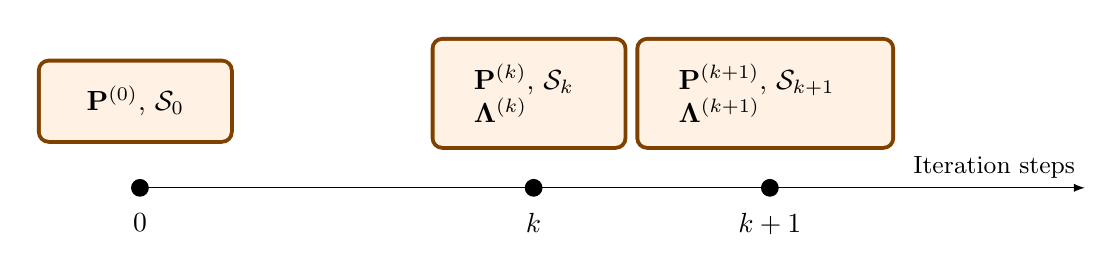
\begin{tikzpicture}
      \draw[-latex] (0,0) -- (12,0) node[above left] {\small Iteration steps};
      \filldraw (0,0) circle (3pt); % Marker
      \filldraw (5,0) circle (3pt); % Marker
      \filldraw (8,0) circle (3pt); % Marker
      \node[align=center] at (0,1.1) {
        \begin{tcolorbox}[colframe=orange!50!black, colback=orange!10, coltitle=black, rounded corners,width=2.5cm]
          \centering $\mathbf P^{(0)}$, $\mathcal S_0$
        \end{tcolorbox}
      };
      \node[align=center,below] at (0,-0.2) {$0$};
      \node[align=center] at (5,1.2) {\begin{tcolorbox}[colframe=orange!50!black, colback=orange!10, coltitle=black, rounded corners,width=2.5cm]
          $\small \mathbf P^{(k)}$, $\mathcal S_{k}$ \\  $\mathbf \Lambda^{(k)}$
        \end{tcolorbox}
      };
      \node[align=center, below] at (5,-0.2) {$k$};
      \node[align=center] at (8,1.2) {\begin{tcolorbox}[colframe=orange!50!black, colback=orange!10, coltitle=black, rounded corners,width=3.3cm]
          $\mathbf P^{(k+1)}$, $\mathcal S_{k+1}$ \\  $\mathbf \Lambda^{(k+1)}$
        \end{tcolorbox}
      };
      \node[align=center,below] at (8,-0.2) {$k+1$};
    \end{tikzpicture}
  \end{center}
  The effectiveness of the algorithm lies in that it is much easier to establish a $q$-dimensional starting subspace which is close to $\text{span}(\mathbf p_1, \dots, \mathbf p_{n_{modes}})$ than to find $n_{modes}$ vectors that are each close to a required eigenvector $\mathbf p_i$.
\end{frame}

\begin{frame}{Preliminary considerations}
  \begin{itemize}
    \item  All characteristics of the Ritz analysis pertain also to the subspace iteration; i.e., the smallest eigenvalues are approximated best in the iteration, and all eigenvalue approximations are \textbf{upper bounds} on the actual eigenvalues sought.
    \item Because the iteration is performed on a subspace, \textbf{convergence of the subspace} is all that is required and not convergence of individual iteration vectors to eigenvectors.
    \item If the initial vectors are linear combinations of the required eigenvectors, the solution algorithm converges in one step.
  \end{itemize}
\end{frame}

\begin{frame}{Pseudo-code of the subspace iteration method}
  \small
  \textbf{Inputs:}
  \begin{itemize}
    \item \(\mathbf K \), \(\mathbf M \): stiffness and mass matrices of large  dimension \( n \times n \).
    \item \( n_{modes} \): number of desired eigenmodes.
    \item \( q \): number of iteration vectors, with \( q > n_{modes} \).
    \item \(\mathbf P^{(0)} \in \mathbb{R}^{n \times q} \): initial guess matrix of linearly independent vectors
          $$\mathbf  P^{(0)}=[\mathbf p^{(0)}_1,\dots,\mathbf p^{(0)}_q]$$
    \item \( \sigma \): spectral shift (optional)
    \item \( \varepsilon \): convergence tolerance
  \end{itemize}

  \textbf{Output:}
  \begin{itemize}
    \item  Approximated eigenvectors: $\mathbf  P^{(k)}=[\mathbf p^{(k)}_1,\dots,\mathbf p^{(k)}_q]$
    \item Approximated eigenvalues: $\mathbf \Lambda^{(k)}=\text{diag}(\lambda^{(k)}_1,\dots,\lambda^{(k)}_q)$
  \end{itemize}
\end{frame}

\begin{frame}{Pseudo-code of the subspace iteration method}
  \small \textbf{Algorithm:}
  \begin{enumerate}
    \item If $\mathbf K$ is singular, use shift: set \( \mathbf K_\sigma =\mathbf K + \sigma\mathbf M \)
    \item For \( k = 1, 2, \dots \) until convergence:
          \begin{itemize}
            \item Do step 1: perform inverse iteration on \( q \) vectors to obtain
                  $$\overline{\mathbf P^{(k)}}.$$
            \item Do step 2a: compute the projected stiffness and mass matrices using $\overline{\mathbf P^{(k)}}$:
                  $$\mathbf K^{(k)} \qquad\text{and}\qquad \mathbf M^{(k)}.$$
            \item Do step 2b: solve the projected \emph{small} generalized eigenvalue problem to obtain the projected modal matrix and the spectral matrix:
                  $$\mathbf Z^{(k)} \qquad\text{and}\qquad \mathbf \Lambda^{(k)}.$$

            \item Do step 2c: calculate the updated modal matrix \( \mathbf P^{(k)} \).
            \item Do step 3: check convergence
          \end{itemize}
  \end{enumerate}
\end{frame}


\begin{frame}{Subspace iteration steps}
  \begin{enumerate}
    \item \textbf{Step 1:} Inverse iteration on \( q \) vectors: find the $(n\times q)$ matrix $\overline{\mathbf P^{(k)}}$ such that
          \[
            \mathbf K\overline{\mathbf P^{(k)}} = \mathbf M\mathbf P^{(k-1)}
          \]
    \item \textbf{Step 2a:} Compute projected stiffness and mass matrices (\(q\times q\)):
          \[
            \mathbf K^{(k)} = (\overline{\mathbf P^{(k)}})^T \mathbf K \overline{\mathbf P^{(k)}}, \quad \mathbf M^{(k)} = (\overline{\mathbf P^{(k)}})^T \mathbf M \overline{\mathbf P^{(k)}}
          \]
    \item \textbf{Step 2b:} Solve the \emph{small} $(q\times q)$ generalized eigenvalue problem: find the projected modal matrix $\mathbf Z^{(k)}$ and the spectral matrix $\mathbf \Lambda^{(k)}$ such that
          \[
            \mathbf K^{(k)}\mathbf Z^{(k)} = \mathbf M^{(k)}\mathbf Z^{(k)} \mathbf \Lambda^{(k)}
          \]
    \item \textbf{Step 2c:} Calculate the updated modal matrix (\(n\times q\)):
          \[
            \mathbf P^{(k)} = \overline{\mathbf P^{(k)}} \mathbf Z^{(k)}
          \]
  \end{enumerate}
\end{frame}

\begin{frame}{Step 1 - Inverse iteration on \( q \) vectors}
  Suppose that the Step 1 is replace by a simultaneous inverse iteration on \( q \) eigenvectors:
  \[
    \mathbf P^{(k)} = (\mathbf K^{-1}\mathbf M)\mathbf P^{(k-1)}=\dots = (\mathbf K^{-1}\mathbf M)^k\, \mathbf P^{(0)}
  \]
  \vspace{-0.5cm}
  \begin{block}{}
    Define the subspace \( \mathcal S^{(k)} \) of rank \( q \), spanned by the vectors \( \{\mathbf p_i^{(k)}\} \).  $\mathbf  P^{(k)}=[\mathbf p^{(k)}_1,\dots,\mathbf p^{(k)}_q]$ forms a \emph{non-orthogonal} basis of \( \mathcal S^{(k)} \).
  \end{block}
  \begin{itemize}
    \item[\XSolidBrush] All columns of \(\mathbf  P^{(k)} \) tend toward \( \mathbf  p_1 \)
    \item[\XSolidBrush]  Collinearity if no orthogonalization is applied !
  \end{itemize}

  \begin{tcolorbox}[colback=darkred!10,colframe=darkred!40!black]
    \begin{center}
      \textbf{Orthogonalization} of vectors \(\mathbf p_i^{(k)} \) at each iteration needed !
    \end{center}
  \end{tcolorbox}
\end{frame}

\begin{frame}{Modified Step 2 - Gram-Schmidt orthogonalization}
  \begin{enumerate}
    \item \textbf{Step 1:} Inverse iteration on \( q \) vectors: find the $(n\times q)$ matrix $\overline{\mathbf P^{(k)}}$ such that
          \[
            \mathbf K\overline{\mathbf P^{(k)}} = \mathbf M\mathbf P^{(k-1)}
          \]
    \item \textbf{Step 2:} Grand-Schmidt orthogonalization:
          $$\mathbf P^{(k+1)}=\mathbf P^{(k)}\mathbf R^{k}$$
          where $\mathbf R^{k}$ is an upper triangular matrix chosen in such way that
          $$(\mathbf P^{(k+1)})^T\mathbf M \mathbf P^{(k+1)} = \mathbf I$$
  \end{enumerate}
  \begin{block}{}
    Gram-Schmidt method is inefficient as iteration vector $\mathbf p_i^{(k)}$ is forced to converge to a prescribed eigenvector $\mathbf p_i$ without allowing a more effective linear combination of the iteration vectors to take place.
  \end{block}
\end{frame}

\begin{frame}{Step 2 - Orthogonalization by minimization of the Rayleigh quotient}
  \begin{itemize}
    \item Orthogonalization by minimization of the Rayleigh quotient:
          \[
            \mathcal R(\mathbf w^{(k)}) = \frac{(\mathbf w^{(k)})^T\mathbf  K \mathbf w^{(k)}}{(\mathbf w^{(k)})^T\mathbf  M\mathbf  w^{(k)}}
          \]
    \item Let \(\mathbf  w^{(k)} = \overline{\mathbf P^{(k)}}\mathbf z^{(k)} \)
    \item Projected Rayleigh's quotient:
          \[
            \mathcal R(\mathbf w^{(k)}) = \frac{(\mathbf z^{(k)})^T\mathbf K^{(k)} \mathbf z^{(k)}}{(\mathbf z^{(k)})^T\mathbf M^{(k)}\mathbf z^{(k)}}
          \]
          where
          \[
            \mathbf K^{(k)} = (\overline{\mathbf P^{(k)}})^T \mathbf K \overline{\mathbf P^{(k)}}, \quad\mathbf M^{(k)} = (\overline{\mathbf P^{(k)}})^T\mathbf M \overline{\mathbf P^{(k)}}
          \]
  \end{itemize}
\end{frame}

\begin{frame}{Step 2b - Solve projected generalized eigenvalue problem}
  \begin{itemize}
    \item Minimization of the projected Rayleigh's quotient (generalized eigenvalue problem of dimension \( q \times q \))
    \item Stationary condition:
          \[
            \delta \mathcal R(\mathbf w^{(k)}) = 0\qquad \Rightarrow\qquad \mathbf K^{(k)} \mathbf z^{(k)} = \lambda^{(k)}\mathbf  M^{(k)}\mathbf  z^{(k)}
          \]

    \item Solve via transformation method (e.g., Jacobi method):
          \[
            \mathbf K^{(k)} \mathbf Z^{(k)} =\mathbf  M^{(k)}\mathbf  Z^{(k)} \mathbf \Lambda^{(k)}
          \]
    \item Ritz vectors and values:
          \[
            \mathbf Z^{(k)} = [\mathbf z_1^{(k)}, \dots,\mathbf  z_q^{(k)}], \quad\text{and}\quad
            \mathbf \Lambda^{(k)} = \text{diag}(\mathbf \lambda_1^{(k)}, \dots, \mathbf \lambda_q^{(k)})
          \]
  \end{itemize}
\end{frame}

\begin{frame}{}
  \textbf{Step 2c - Update modal matrix and orthogonality check}
  \vspace{0.3cm}
  \begin{itemize}
    \item Update the modal matrix:
          $$\mathbf P^{(k)} = \overline{\mathbf P^{(k)}} \mathbf Z^{(k)}$$
    \item Orthogonality check:
          \[
            (\mathbf P^{(k)})^T\mathbf M\mathbf P^{(k)} =\mathbf I
          \]
  \end{itemize}

  \textbf{Step 3 - Convergence to stop iteration}\newline
  Convergence criterion based on relative change of eigenvalues:
  \[
    \frac{|\lambda_i^{(k)} - \lambda_i^{(k-1)}|}{\lambda_i^{(k)}} < \varepsilon, \quad i = 1, 2, \dots, n_{modes}
  \]
\end{frame}


\begin{frame}{Starting iteration vectors $\mathbf P^{(0)}$}
  \begin{itemize}
    \item The starting iteration vectors in $\mathbf P^{(0)}$ should not be too close to each other, i.e., they should be linearly independent.
    \item Higher convergence rate can be obtained by increasing $q$. However, using more iteration vectors will also increase the computer effort for one iteration. In practice
          $$q=\min(2n_{modes},\, n_{modes} + 8)$$
  \end{itemize}
  \begin{tcolorbox}[colback=darkred!10,colframe=darkred!40!black]
    \textbf{Empirical guidelines}
    \begin{itemize}
      \item The first column of $\mathbf P^{(0)}$ should be the diagonal of $\mathbf M$. This ensures that all mass degrees of freedom are excited.
      \item The other columns in $\mathbf P^{(0)}$, except for the last column, should be unit vectors $\mathbf e_i$, with entries $+1$ at the degrees of freedom with the smallest ratios $k_{ii}/m_{ii}$, and the last column in $\mathbf P^{(0)}$ should be a random vector with values in $[0,1]$.
    \end{itemize}
  \end{tcolorbox}
\end{frame}

\begin{frame}{Convergence of the subspace iteration method}
  \begin{itemize}
    \item Iteration is performed with $q$ vectors, $q > n_{modes}$, but convergence is measured only on the approximations obtained for the $n_{modes}$ smallest eigenvalues.
    \item If the starting iteration vectors in $\mathbf P^{(0)}$, are not orthogonal to any one of the required eigenvectors $\mathbf p_1,\dots, \mathbf p_{n_{modes}}$, then as $k\to \infty$
          $$\tilde{\mathcal S}_k=\text{span}(\mathbf p^{(k)}_1, \dots, \mathbf p^{(k)}_{n_{modes}})\to \mathcal S_\infty = \text{span}(\mathbf p_1, \dots, \mathbf p_{n_{modes}})$$\
    \item  Assuming that in the iteration
          the vectors in $\mathbf P^{(k+1)}$ are ordered in such way that the $i$-th diagonal element in $\mathbf \Lambda^{(k+1)}$ is larger
          than the $(i - 1)$-st element for $i = 2,\dots, p$, then the $i$-th column in $\mathbf P^{(k+1)}$ converges to $\mathbf p_i$ and the convergence rate is
          $$\lambda_i/\lambda_{p+1}$$
          Although this is an asymptotic convergence rate, it indicates that the smallest eigenvalues converge fastest.
  \end{itemize}
\end{frame}

\begin{frame}{Final Sturm sequence check}
  \begin{block}{}
    After convergence is achieved, a final check based on the Sturm sequence property can be performed to ensure that the number of computed eigenvalues below a certain value is correct.
  \end{block}

  \begin{itemize}
    \item The Sturm sequence property states that the number of eigenvalues of the generalized eigenvalue problem \( \mathbf K\mathbf p = \lambda\mathbf M \mathbf p \) that are less than a given value \( \lambda^* \) is equal to the number of negative pivots obtained when performing an \( \mathbf L\mathbf  D\mathbf  L^T \) factorization of the matrix \( \mathbf K - \lambda^* \mathbf M \).
    \item This property can be used to verify that the number of computed eigenvalues below a certain threshold matches the expected count, providing an additional layer of validation for the results obtained from the subspace iteration method.
  \end{itemize}
\end{frame}

\section{The Lanczos algorithm}

\begin{frame}{Lanczos and subspace iteration}
  \small
  Both methods reuse a stiffness factorization and use Rayleigh--Ritz
  extraction to approximate the lowest modes of
  $\mathbf K\mathbf p=\lambda\mathbf M\mathbf p$.

  \medskip
  \centering
  \renewcommand{\arraystretch}{1.32}
  \begin{tabular}{@{}>{\raggedright\arraybackslash}p{.18\linewidth}
    >{\raggedright\arraybackslash}p{.37\linewidth}
    >{\raggedright\arraybackslash}p{.37\linewidth}@{}}
    \rowcolor{darkred!15}
                                                                       & \textbf{Subspace iteration} & \textbf{Scalar Lanczos} \\
    \textbf{Trial space}                                               &
    Update a block of $q$ vectors together. Its dimension stays fixed. &
    Start with one vector. Append one new direction per step within a stage.                                                   \\[5pt]
    \textbf{Stiffness solves}                                          &
    $q$ right-hand sides per outer iteration.                          &
    One right-hand side per new direction.                                                                                     \\[5pt]
    \textbf{Reduced problem}                                           &
    Project $\mathbf K$ and $\mathbf M$. Solve a generally dense
    $q\times q$ generalized eigenproblem.                              &
    Project the inverse operator. Solve a symmetric tridiagonal
    standard eigenproblem.                                                                                                     \\
  \end{tabular}
\end{frame}

\begin{frame}{Why inverse Lanczos targets the lowest frequencies}
  \small
  Assume $\mathbf K$ and $\mathbf M$ are symmetric positive definite.
  The inverse operator $\mathbf A=\mathbf K^{-1}\mathbf M$ preserves the
  mode shapes and reverses the ordering of the eigenvalues.
  \[
    \mathbf K\mathbf p_i=\lambda_i\mathbf M\mathbf p_i
    \quad\Longrightarrow\quad
    \mathbf A\mathbf p_i=\frac{1}{\lambda_i}\,\mathbf p_i,
    \qquad \lambda_i=\omega_i^2 .
  \]
  Thus each application of $\mathbf A$ amplifies the lowest modes most
  strongly relative to the others.

  \begin{block}{Building the trial space}
    Choose a starting shape with components in the modes of interest.
    Normalize it to $\mathbf v_1^T\mathbf M\mathbf v_1=1$. After $m$ steps,
    the Lanczos basis spans the Krylov subspace
    \[
      \mathcal K_m(\mathbf A,\mathbf v_1)
      =\operatorname{span}\{\mathbf v_1,\mathbf A\mathbf v_1,\ldots,
      \mathbf A^{m-1}\mathbf v_1\}.
    \]
  \end{block}
  Factor $\mathbf K$ once. Apply $\mathbf A$ by solving
  $\mathbf K\mathbf z=\mathbf M\mathbf v_j$ with the stored factors.
\end{frame}

\begin{frame}{One Lanczos step}
  \small
  Set $\mathbf v_0=\mathbf 0$ and $\beta_0=0$. Given the mass-normalized
  vector $\mathbf v_j$, compute the next direction as follows.
  \begin{enumerate}
    \item \textbf{Apply the inverse operator.}\quad
          Solve $\mathbf K\mathbf z=\mathbf M\mathbf v_j$.
    \item \textbf{Remove the components along the last two directions.}
          \[
            \alpha_j=\mathbf v_j^T\mathbf M\mathbf z,\qquad
            \mathbf w=\mathbf z-\alpha_j\mathbf v_j-\beta_{j-1}\mathbf v_{j-1}.
          \]
          In exact arithmetic $\mathbf w$ is already mass-orthogonal to all
          earlier vectors. In floating-point arithmetic, reorthogonalize as needed.
    \item \textbf{Normalize the new direction.}
          \[
            \beta_j=\sqrt{\mathbf w^T\mathbf M\mathbf w},\qquad
            \mathbf v_{j+1}=\mathbf w/\beta_j \quad(\beta_j>0).
          \]
          If $\beta_j=0$, the current space is invariant. End this stage.
  \end{enumerate}
\end{frame}

\begin{frame}{From the tridiagonal matrix to the physical modes}
  \small
  Collect the trial vectors in $\mathbf V_m=[\mathbf v_1,\ldots,\mathbf v_m]$.
  Their mass orthogonality gives $\mathbf V_m^T\mathbf M\mathbf V_m=\mathbf I$.
  Rayleigh--Ritz projection of the inverse operator gives
  \[
    \mathbf T_m=\mathbf V_m^T\mathbf M\mathbf A\mathbf V_m
    =\begin{bmatrix}
      \alpha_1 & \beta_1  &             & 0           \\
      \beta_1  & \alpha_2 & \ddots      &             \\
               & \ddots   & \ddots      & \beta_{m-1} \\
      0        &          & \beta_{m-1} & \alpha_m
    \end{bmatrix}.
  \]
  The recurrence supplies every entry. Solve
  $\mathbf T_m\mathbf s_i=\nu_i\mathbf s_i$ with $\|\mathbf s_i\|_2=1$.
  \begin{block}{Recover the lowest frequencies from the largest Ritz values $\nu_i$}
    \[
      \lambda_i=\frac{1}{\nu_i},\qquad
      {\mathbf p}_i=\mathbf V_m\mathbf s_i .
    \]
  \end{block}
\end{frame}

\begin{frame}{When have the requested modes converged?}
  \small
  For a unit eigenvector $\mathbf s_i$ of $\mathbf T_m$, the last component
  $(\mathbf s_i)_m$ gives a residual check from quantities already available.
  In exact arithmetic, with $\|\mathbf x\|_{\mathbf M}^2=\mathbf x^T\mathbf M\mathbf x$,
  \[
    \|\mathbf A{\mathbf p}_i-\nu_i{\mathbf p}_i\|_{\mathbf M}
    =|\beta_m(\mathbf s_i)_m|.
  \]
  \begin{enumerate}
    \item \textbf{Check each mode.} Test this residual against the chosen
          tolerance and verify equilibrium in the original model using
          ${\mathbf r}_i=\mathbf K{\mathbf p}_i-\lambda_i\mathbf M{\mathbf p}_i$.
    \item \textbf{Continue or restart.} If more modes are needed when the
          stage ends, keep the converged modes. Restart with a new vector
          mass-orthogonal to them. Reorthogonalization helps prevent duplicate modes.
    \item \textbf{Check completeness.} A single starting vector can capture
          only one direction per repeated eigenspace. At a cutoff $\omega^*$,
          count the eigenvalues below $\lambda^*=(\omega^*)^2$ using the Sturm check.
  \end{enumerate}
\end{frame}

\end{document}
